\section{Calendar}
\label{sec:calendar}

The calendar is a new feature in \salespoint{} to manage appointments and events.
Figure~\ref{calendar_overview} shows the UML model of the calendar.

\begin{figure}[ht]
	\centering
  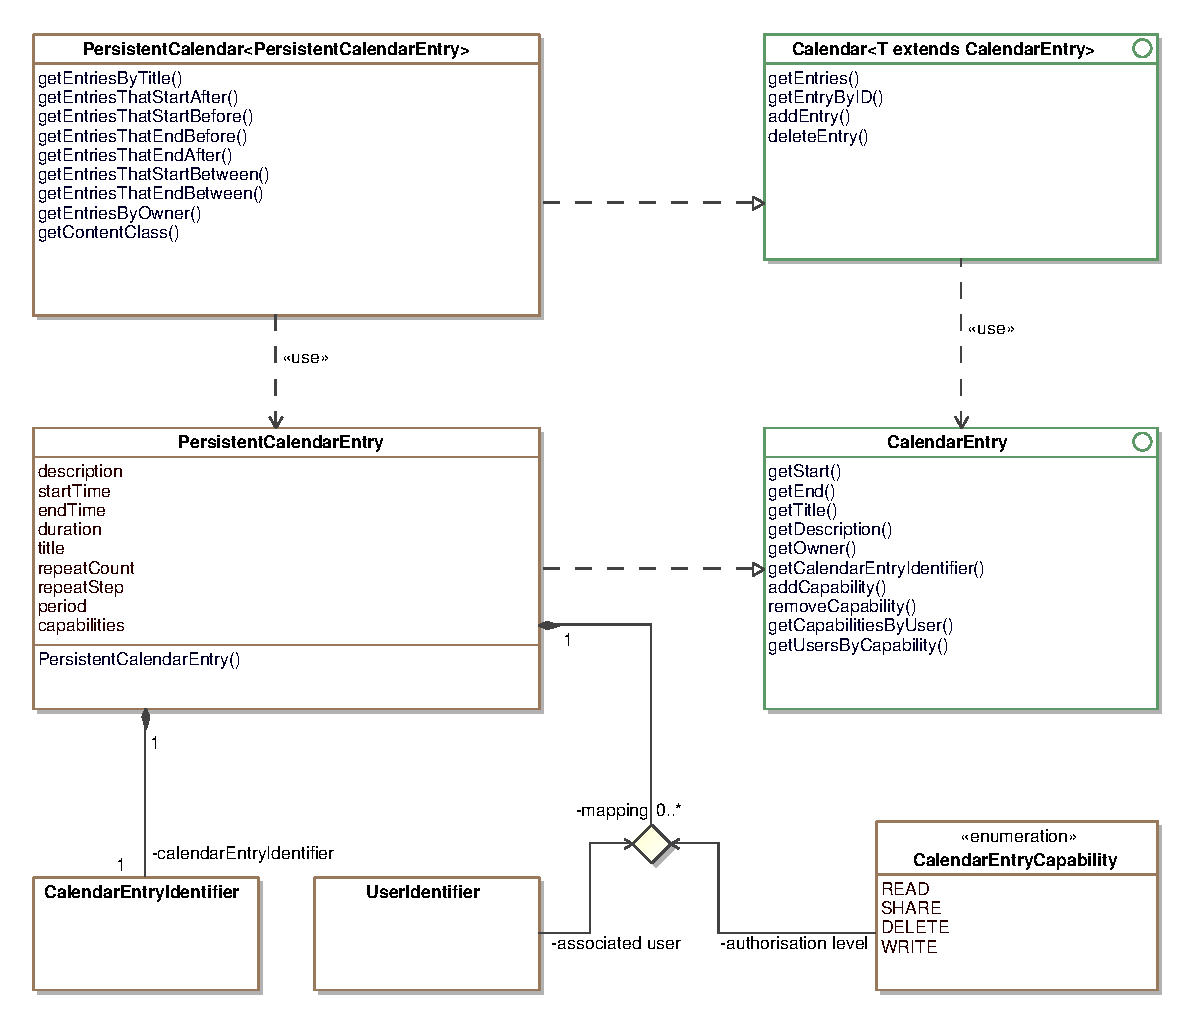
\includegraphics[width=1.0\textwidth]{images/Calendar_Overview.eps}
	\label{calendar_overview}
	\caption{Calendar - Class Overview}
\end{figure}

\code{Calendar} is an interface that provides simple functionality to store and retrieve \code{CalendarEntry}s.
\code{CalendarEntry} is an interface to set, store and access information of a single appointment/event.
Both interfaces are implemented by \code{PersistentCalendar} and \code{PersistentCalendarEntry}, respectively.
\code{PersistentCalendarEntry} is a persistence entity containing all information and \code{PersistentCalendar} manages the JPA access.
\\

Every calendar entry is uniquely identified by a \code{CalendarEntryIdentifier}.
This identifier also serves as primary key attribute when persisting an entry to the database.
Additionally, a \code{PersistentCalendarEntry} must have an owner, a title, a start and an end date.
The user who created the entry is known as the owner and identified by \code{ownerID} of the type \code{UserIdentifier}.
\\

The access of other users than the owner to a calendar entry is restricted by capabilities.
For each calendar entry, a user identifier and a set of capabilities are stored.
Possible capabilities are:
\begin{itemize}
    \item \code{READ} - indicates if a user can read this entry
    \item \code{WRITE} - indicates if a user can change this entry
    \item \code{DELETE} - indicates if a user can delete this entry
    \item \code{SHARE} - indicates if a user can share this entry with other users
\end{itemize}.

Because \salespoint{} only implements the model of the MVC pattern (see Section~\ref{spring}), the developer has to check and enforce capabilities in the controller.
\\

Besides the minimum information of owner, title, start and end a calendar entry can also have a description, which may contain more information.
Periodic appointments are also supported, by specifing the number of repetitions (\code{count} in Figure~\ref{calendar_overview}) and a time span between two appointments (\code{period} in Figure~\ref{calendar_overview}).
\\

There are some conditions for temporal attributes of an calendar entry:
\begin{itemize}
    \item the start must not be after the end
    \item the time between two repetitions of an appointment need to be longer than the duration of the appointment, so that appointments do not overlap
\end{itemize}
%All attributes of the entry can be changed, except of the owner, who will be defined when the entry is created and then becomes immutable. 
